\section{Kết quả thử nghiệm thực tế trên tài khoản học sinh Vuong}\label{sec:eval-trial}

Mục này đọc nhật ký tài khoản Vuong để trả lời: học sinh đã làm bao nhiêu câu, các câu kết thúc ra sao, gia sư đã giúp bao nhiêu và vòng dạy có chạy đủ các bước không. Bảng~\ref{tab:db-overview} cho quy mô trên các buổi có ít nhất một câu được hiển thị: tài khoản học $523$ câu và gửi $726$ câu trả lời đã chấm, trong đó Toán chiếm $89{,}9\%$ số câu. Chín trong mười buổi Toán diễn ra trong hai ngày 12 và 13/10, khi chủ dự án cho tài khoản học hết các tình huống của hai chương; hai buổi Tiếng Anh cách đó một tháng, sau khi môn thứ ba được thêm vào hệ thống.

% Sinh bởi tools/db_tex.py từ bản sao lưu database; không sửa tay.
\begin{table}[H]
\centering
\caption{Quy mô dữ liệu thử nghiệm đọc từ database}\label{tab:db-overview}
\begin{tabular}{lrrr}
\toprule
Chỉ số & Số thập phân & Diện tích & Tiếng Anh \\
\midrule
Số buổi học đã ghi & $10$ & $6$ & $5$ \\
Số buổi có nội dung & $6$ & $4$ & $3$ \\
Số buổi đã hoàn thành & $5$ & $3$ & $2$ \\
Số tài khoản thử nghiệm & $1$ & $1$ & $1$ \\
Số sự kiện & $5\,791$ & $3\,528$ & $1\,906$ \\
Số câu hỏi đã hiển thị & $287$ & $183$ & $53$ \\
Số lượt trả lời đã chấm & $401$ & $251$ & $74$ \\
Số câu đã giải quyết & $286$ & $182$ & $52$ \\
\bottomrule
\end{tabular}
\end{table}


\subsection{Các câu kết thúc ra sao}
Bảng~\ref{tab:db-results} và Hình~\ref{fig:db-resolution} cho cách các câu kết thúc. Học sinh tự làm được $58{,}4\%$ số câu ở chương Số thập phân, $64{,}3\%$ ở chương Diện tích và $76{,}9\%$ ở Unit~11. Phần còn lại chủ yếu được giải quyết sau gợi ý ($32{,}9\%$, $30{,}2\%$ và $19{,}2\%$) và chỉ một phần nhỏ phải làm mẫu ($5{,}6\%$, $3{,}8\%$ và $1{,}9\%$). Câu chưa giải quyết chỉ chiếm $3{,}1\%$, $1{,}6\%$ và $1{,}9\%$, nên gia sư đưa gần mọi câu đến đáp án đúng, có hoặc không có giúp đỡ. Số gợi ý trung bình cho mỗi câu giảm từ $0{,}71$ ở Số thập phân xuống $0{,}54$ ở Diện tích và $0{,}52$ ở Unit~11.

% Sinh bởi tools/db_tex.py từ bản sao lưu database; không sửa tay.
\begin{table}[H]
\centering
\caption{Cách giải quyết câu và kết quả chấm từng lượt trả lời}\label{tab:db-results}
\begin{tabular}{lrrr}
\toprule
Chỉ số & Số thập phân & Diện tích & Tiếng Anh \\
\midrule
Tự làm & $167$ ($58{,}4$\%) & $117$ ($64{,}3$\%) & $40$ ($76{,}9$\%) \\
Có gợi ý & $94$ ($32{,}9$\%) & $55$ ($30{,}2$\%) & $10$ ($19{,}2$\%) \\
Làm mẫu & $16$ ($5{,}6$\%) & $7$ ($3{,}8$\%) & $1$ ($1{,}9$\%) \\
Chưa giải quyết & $9$ ($3{,}1$\%) & $3$ ($1{,}6$\%) & $1$ ($1{,}9$\%) \\
\midrule
Đúng & $273$ ($68{,}1$\%) & $179$ ($71{,}3$\%) & $50$ ($67{,}6$\%) \\
Đúng một phần & $0$ ($0{,}0$\%) & $0$ ($0{,}0$\%) & $3$ ($4{,}1$\%) \\
Sai & $128$ ($31{,}9$\%) & $72$ ($28{,}7$\%) & $21$ ($28{,}4$\%) \\
\midrule
Số lần thử trung bình mỗi câu & $1{,}40$ & $1{,}37$ & $1{,}42$ \\
Số gợi ý trung bình mỗi câu & $0{,}71$ & $0{,}54$ & $0{,}52$ \\
\bottomrule
\end{tabular}
\end{table}


\begin{figure}[H]
\centering
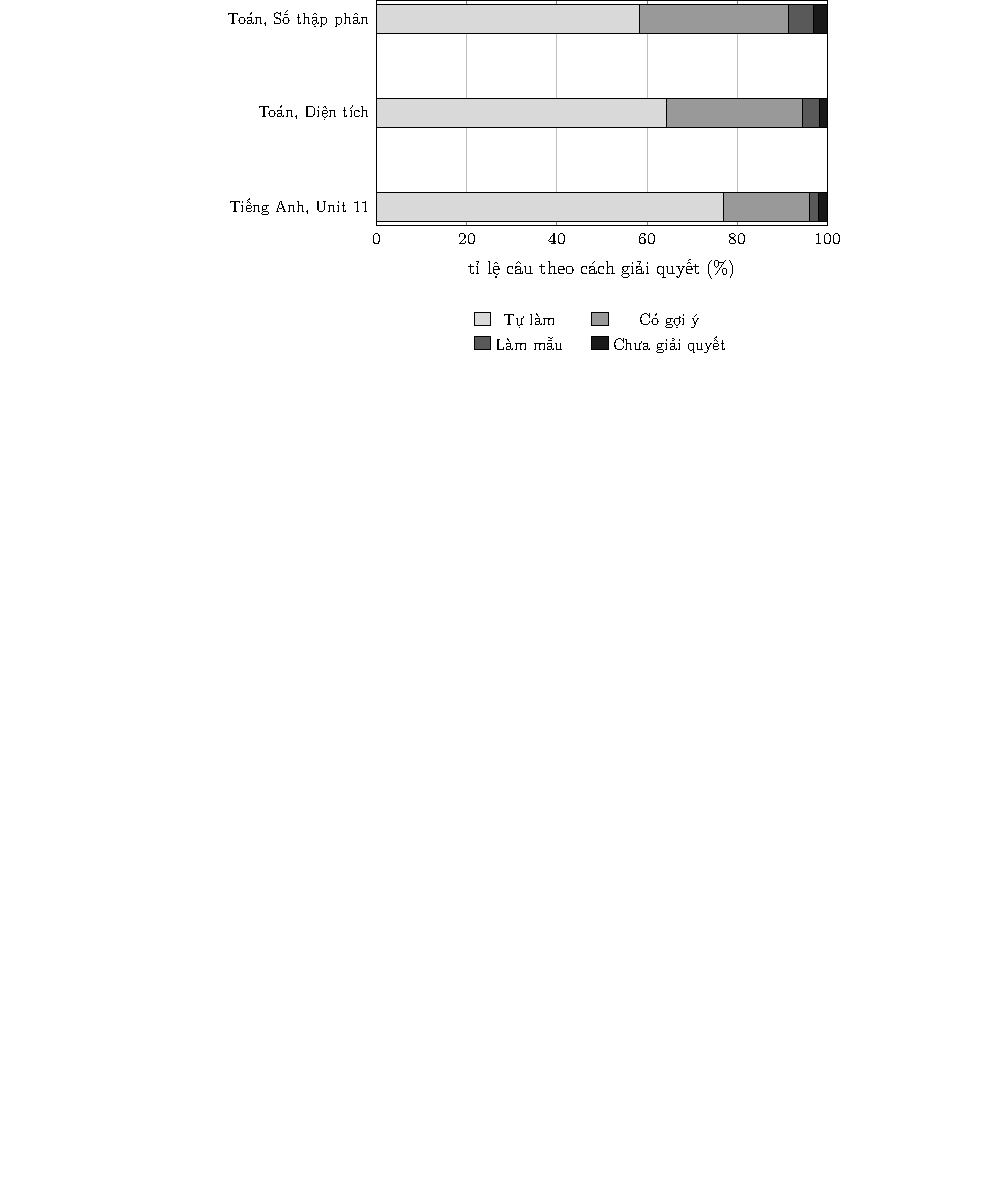
\includegraphics{figures/pdf/fig-db-resolution.pdf}
\caption{Tỉ lệ câu theo cách kết thúc của tài khoản Vuong ở ba nội dung. Mỗi thanh cộng lại bằng $100\%$.}
\label{fig:db-resolution}
\end{figure}

Hình~\ref{fig:db-curve} vẽ tỉ lệ câu tự làm của từng buổi từ tám câu trở lên theo thứ tự thời gian. Chương Diện tích tăng đều từ $41{,}7\%$ ở buổi đầu lên $53{,}7\%$, $70{,}7\%$ và $72{,}4\%$ ở ba buổi sau. Chương Số thập phân đi từ $52{,}4\%$ ở buổi hoàn chỉnh đầu tiên lên $66{,}7\%$ ở buổi thứ năm rồi giảm xuống $51{,}5\%$ ở buổi cuối; buổi cuối chỉ có $33$ câu nên dao động lớn và số liệu không đủ để nói nguyên nhân. Hai buổi Tiếng Anh có mức tự làm cao ngay từ đầu ($78{,}0\%$ và $72{,}7\%$) nhưng chỉ có $41$ và $11$ câu nên chưa so được với Toán.

\begin{figure}[H]
\centering
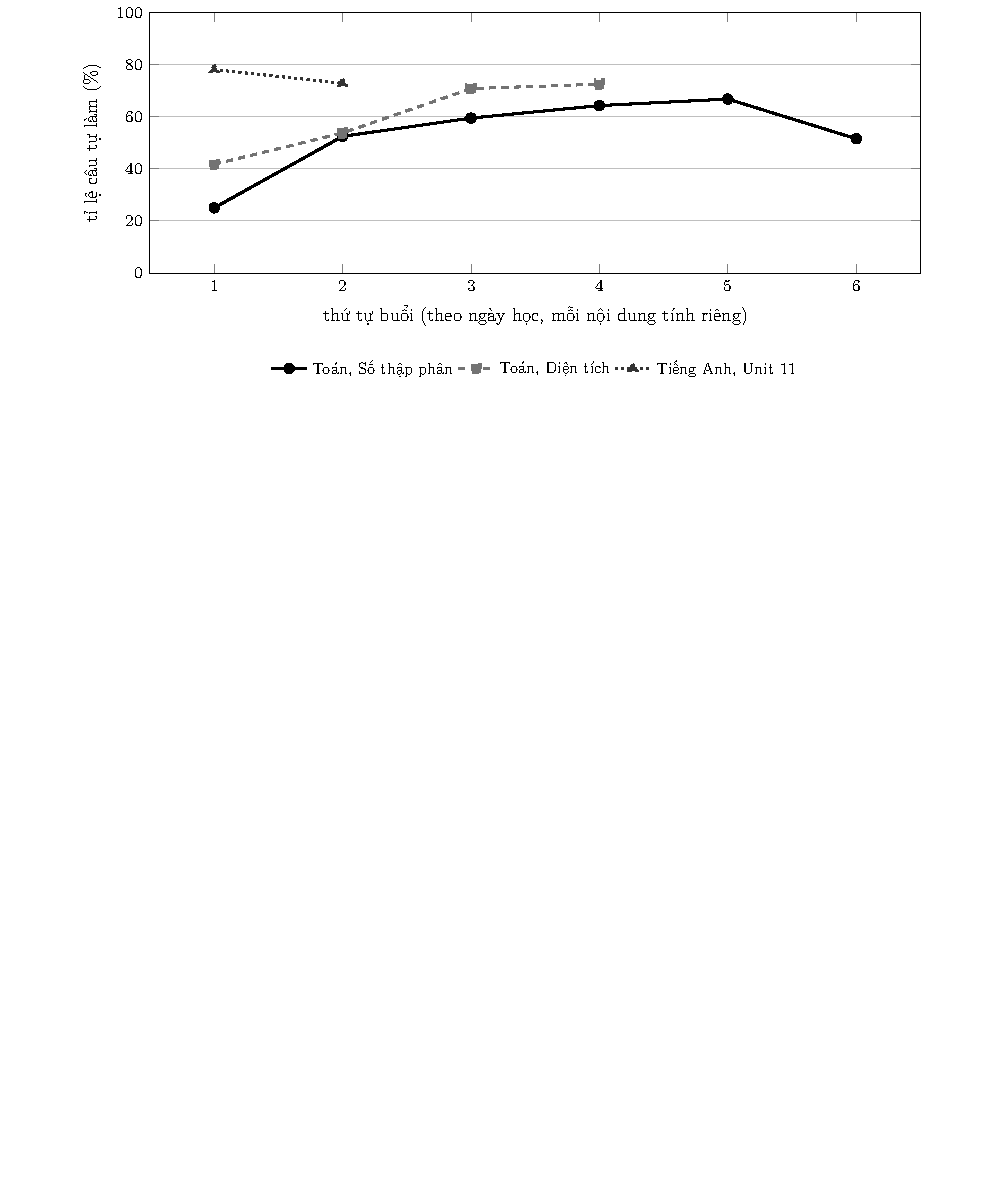
\includegraphics{figures/pdf/fig-db-curve.pdf}
\caption{Tỉ lệ câu tự làm của tài khoản Vuong theo thứ tự buổi, mỗi nội dung một đường; chỉ tính các buổi từ tám câu trở lên.}
\label{fig:db-curve}
\end{figure}

\subsection{Gợi ý theo bậc và vòng dạy}
Gợi ý tập trung ở bậc thấp, đúng nguyên tắc Socratic. Môn Toán có $295$ gợi ý: $62{,}7\%$ ở bậc một, $19{,}7\%$ ở bậc hai, $4{,}4\%$ ở bậc ba và $13{,}2\%$ là làm mẫu (bậc sáu và bảy); chỉ khoảng một trong tám gợi ý đi đến làm mẫu. Môn Tiếng Anh có $28$ gợi ý trải đều hơn trên các bậc một đến ba. Học sinh chủ động xin gợi ý $37$ lần ở Số thập phân, $16$ lần ở Diện tích và $10$ lần ở Unit~11, ít hơn tổng gợi ý đã đưa, nên phần lớn gợi ý do chính sách quyết định chứ không do học sinh đòi. Về vòng dạy, học sinh vào bài $47$ lần và qua bài $44$ lần ($93{,}6\%$) ở Số thập phân, vào $27$ lần và qua $26$ lần ($96{,}3\%$) ở Diện tích; Tiếng Anh qua $6$ trên $9$ lần vào bài, mẫu quá nhỏ và là buổi đầu của một môn mới đang sửa lỗi. Các quyết định dạy lý thuyết, hỏi kể lại, làm mẫu và đưa câu luyện tập xuất hiện đủ trong nhật ký cả hai môn, nên vòng sáu bước chạy trọn vẹn thay vì rút gọn thành một chuỗi câu hỏi.

\section{Mô hình ngôn ngữ và bộ kiểm chứng trong thực tế}\label{sec:eval-model}
Mục này đếm hoạt động của mô hình ngôn ngữ và bộ kiểm chứng trên cả năm tài khoản. Nó cũng trả lời một câu hỏi của việc đánh giá: mô hình ngôn ngữ thực sự viết bao nhiêu phần phản hồi, khi mỗi nước đi còn có câu mẫu của giáo viên làm dự phòng.

Hình~\ref{fig:db-source} cho biết mỗi phản hồi của gia sư do ai viết: mô hình, câu mẫu của giáo viên hay câu dự phòng khi không có gợi ý hợp lệ. Ở các buổi Toán đầu tháng 10 của Vuong, mô hình chỉ viết $2{,}1\%$ số phản hồi, còn $85{,}6\%$ là câu mẫu và $12{,}3\%$ là câu dự phòng, vì khi đó bộ diễn đạt còn là phiên bản cũ. Tỉ lệ này lên $40{,}9\%$ ở các buổi Toán cuối tháng 10 của những tài khoản khác, sau các đợt cải tiến lời dạy. Ở Tiếng Anh, mô hình viết $34{,}8\%$ phản hồi lần học đầu ngày 15/11 và $68{,}2\%$ lần sau khi sửa chuỗi mô hình và hạn mức gọi. Đây là câu trả lời cho thắc mắc rằng phần lớn lượt dùng câu mẫu chuẩn của giáo viên: điều đó đúng ở bản diễn đạt cũ, và phần của mô hình đã tăng ở các bản sau; câu mẫu vẫn là tuyến dự phòng cuối nên tỉ lệ do mô hình viết không bao giờ đến $100\%$, và đó là chủ ý thiết kế. Trong $13$ kịch bản có kiểm soát ở mục~\ref{sec:eval-socratic}, mô hình viết $26$ trong $31$ lượt ($84\%$) của CAVAT, còn $5$ lượt (nêu đề và đóng câu hỏi) luôn dùng câu mẫu theo thiết kế.

\begin{figure}[H]
\centering
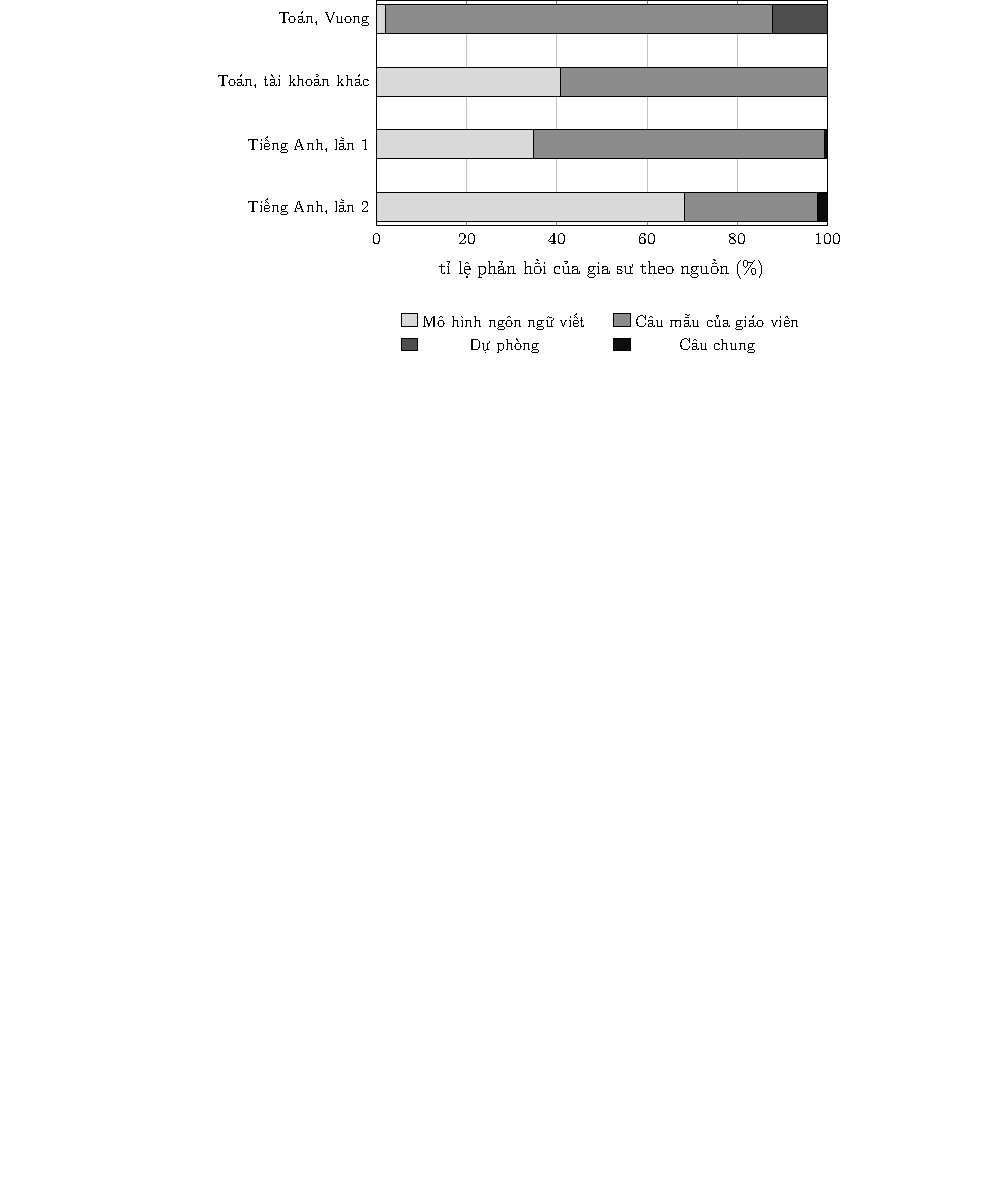
\includegraphics{figures/pdf/fig-db-source.pdf}
\caption{Tỉ lệ phản hồi của gia sư theo nguồn ở bốn nhóm buổi: Toán của Vuong (đầu tháng 10), Toán của bốn tài khoản khác (cuối tháng 10) và hai lần học Tiếng Anh của Vuong ngày 15/11.}
\label{fig:db-source}
\end{figure}

Bốn mô hình nhận $735$ lần gọi: gpt-oss-120b nhiều nhất ($337$ lần), tiếp đến Qwen ($219$), gpt-oss-20b ($155$) và Gemini ($24$); số token vào trung bình mỗi lần gọi từ $1\,321$ đến $1\,753$, thấp hơn nhiều giới hạn $3\,000$. Trong $1\,604$ lần chuyển sang mô hình kế tiếp, nguyên nhân là hết hạn mức ($71{,}1\%$), mô hình không phản hồi ($27{,}9\%$) và chỉ $1{,}0\%$ do kết quả không hợp lệ. Vấn đề chính của chuỗi mô hình vì vậy là hạn mức miễn phí chứ không phải chất lượng đầu ra, và điều đó biện minh cho chuỗi có dự phòng. Về bộ kiểm chứng, Bảng~\ref{tab:db-rejected} đếm lý do từ chối: ở Toán là phản hồi quá dài ($30$ lần), thiếu câu hỏi ($10$) và xưng hô sai ($10$); ở Tiếng Anh là từ tiếng Anh ngoài tư liệu ($20$), lộ đáp án ($8$), nhiều hơn một câu hỏi ($6$) và thiếu câu hỏi ($6$). Tám lần lộ đáp án bị chặn và không lần nào đến học sinh. Hai dòng đầu của bảng ($24$ lần hết số lần gọi và $22$ lần mô hình vẫn không qua kiểm chứng) là các lần hệ thống bỏ lời của mô hình để dùng câu mẫu, nên đo mức rơi về tuyến dự phòng chứ không đo lỗi của gia sư.

% Sinh bởi tools/db_tex.py từ bản sao lưu database; không sửa tay.
\begin{table}[H]
\centering
\caption{Lý do bộ kiểm chứng từ chối phản hồi của gia sư}\label{tab:db-rejected}
\begin{tabular}{lrr}
\toprule
Lý do từ chối & Toán & Tiếng Anh \\
\midrule
quá dài & $30$ & $0$ \\
hết số lệnh gọi của buổi & $0$ & $24$ \\
mô hình vẫn không qua kiểm chứng & $0$ & $22$ \\
từ tiếng Anh ngoài tư liệu của bài & $0$ & $20$ \\
thiếu câu hỏi & $10$ & $6$ \\
xưng hô sai & $10$ & $0$ \\
lộ đáp án & $0$ & $8$ \\
nhiều hơn một câu hỏi & $0$ & $6$ \\
từ ngoài tư liệu của câu & $0$ & $1$ \\
khen trí thông minh & $0$ & $1$ \\
\bottomrule
\end{tabular}
\end{table}

